% 期末作业终局研究备忘：红利低波50ETF 温度计择时策略回测与迭代研究
% 基于 latex 技能 A4 模板（\ChineseMemotrue，xelatex 编译）
\documentclass[a4paper,10pt]{article}
\usepackage[margin=18mm,footskip=9mm]{geometry}
\usepackage{iftex}
\newif\ifChineseMemo
\ChineseMemotrue
\ifChineseMemo
  \ifPDFTeX
    \PackageError{finance-memo}{Chinese text requires XeLaTeX or LuaLaTeX}{}
  \else
    \usepackage[UTF8,fontset=fandol]{ctex}
    \renewcommand{\familydefault}{\sfdefault}
  \fi
\fi
\usepackage{booktabs,graphicx,xcolor,caption,xurl,fancyhdr}
\definecolor{MemoBlue}{HTML}{203E70}
\definecolor{MemoRule}{HTML}{B9C8DF}
\usepackage[colorlinks=true,linkcolor=MemoBlue,urlcolor=MemoBlue]{hyperref}
\captionsetup{font=small,labelfont=bf,skip=4pt}
\setlength{\parindent}{0pt}
\setlength{\parskip}{5pt}
\pagestyle{fancy}
\fancyhf{}
\renewcommand{\headrulewidth}{0pt}
\renewcommand{\footrulewidth}{0.3pt}

\newcommand{\ReportTitle}{红利低波50ETF温度计择时策略：回测与三轮迭代研究}
\newcommand{\ReportType}{研究备忘 · 期末作业}
\newcommand{\ReportDate}{2026 年 11 月 9 日}
\newcommand{\DataDate}{2026 年 8 月 12 日}
\newcommand{\ReportScope}{波段择时策略研究：提出假设→取数→回测→评审→修订→再回测；\\ 窗口 2020-02-26 \textasciitilde{} 2026-08-12，对照买入持有基线}
\newcommand{\TeamName}{邢敏}
\newcommand{\DeskName}{金融人工智能编程 2026 秋\\学号 25260660106}
\newcommand{\ReportAuthor}{邢敏（25 级 FMBA）}
\newcommand{\Coverage}{红利低波50ETF（sh515450）}
\newcommand{\KeyFinding}{最终假设 v2（温度计阈值 80 二元择时）5 条验收标准中 4 条达标，第 2 条（最大回撤）未达标——按验收规则判定未通过，如实呈现。三轮迭代各产出一条被数据证实或证伪的设计知识。}
\fancyfoot[L]{\scriptsize\TeamName}
\fancyfoot[R]{\scriptsize\ReportType}

\begin{document}
\begin{minipage}[t]{0.70\textwidth}
\vspace{0pt}
{\small\ReportDate}\par\medskip
{\color{MemoBlue}\hrule height 0.5pt}\smallskip
{\large\ReportType}\par
{\LARGE\bfseries\ReportTitle}\par\medskip
\ReportScope
\end{minipage}\hfill
\begin{minipage}[t]{0.23\textwidth}
\vspace{0pt}\raggedleft
\colorbox{MemoBlue}{\parbox[c][19mm][c]{0.86\linewidth}{\centering\color{white}\bfseries\TeamName}}\par\medskip
\DeskName
\end{minipage}
\par\bigskip
{\color{MemoBlue}\hrule height 0.5pt}\medskip
{\large\KeyFinding}\par\bigskip

\begin{minipage}[t]{0.61\textwidth}
\vspace{0pt}\raggedright\small
\setlength{\parskip}{4pt}
\textbf{问题与工作流}\par
为周期性重复的策略研究任务设计端到端长程智能体工作流并全程执行：提出假设
→取数→回测→评审→修订→再回测。Controller（确定性状态机）调度；Generator
/Critic（LLM）分别只提假设、只读评审；取数、回测、指标与验收判定均为确定性
代码；人工门禁 H1/H2 把守结构变更与终局。每轮迭代为一个 run：假设、数据
快照哈希、指标、裁决全落盘，可复现可回滚（见 DESIGN.md）。

\textbf{数据与口径}\par
信号：自制温度计（估值+热度+拥挤度，日度，截至 2026-08-12）；行情：
akshare/东方财富后复权日线，上市日 2020-02-26 自动确认（新浪源交叉一致）。
窗口取交集并按信号末日裁切（as\_of 纪律），1566 个交易日；成本：单边万 3
双边、免最低 5 元、无印花税、无滑点；夏普 rf=0、日频年化。

\textbf{发现（事实）}\par
v2 规则：温度 $>$80 清仓、$\leq$80 满仓，t 日判定、t+1 收盘执行，二元仓位。
19 笔卖出全部落在温度尖峰（2020-07、2021-02、2023-05、2024-09-30），四次逃顶
贡献超额：年化 12.55\% 对基线 10.42\%，夏普 1.005 对 0.806。2022-02
\textasciitilde{} 10 慢熊回撤 -13.87\% 与基线完全相同，未达"$\leq$基线
$\times$0.7"的验收线——该区间温度计最高仅 61.1，全程未触发清仓。

\textbf{解读（判断）}\par
温度计为逆向逃顶指标，其热度/拥挤度维度在阴跌市中自然冷却，对慢熊无预警；
三轮迭代证明这是指标能力边界的结构性问题（调参无解、趋势过滤反害），
非某组参数的偶然失手。

\textbf{风险与局限}\par
单窗口样本内评估；无滑点与成本简化或高估收益；温度计为自制指标；完整
清单与诚实结论见第 2 页末。
\end{minipage}\hfill
\begin{minipage}[t]{0.36\textwidth}
\vspace{0pt}\small
% 侧栏包装：表 1 关键数据 + 侧栏小图（caption/来源注记为撰写内容）
\captionof{table}{关键数据：v2 策略与买入持有基线}\label{tab:key-data}
{\footnotesize 同快照、同窗口（2020-02-26 \textasciitilde{} 2026-08-12）、同口径（后复权，含成本）。策略累计净值 2.086，基线 1.851。\par}
\begin{tabular}{lcc}
\toprule
指标 & v2 策略 & 买入持有 \\
\midrule
年化收益 & 12.55\% & 10.42\% \\
最大回撤 & -13.87\% & -13.87\% \\
夏普（rf=0） & 1.005 & 0.806 \\
累计净值 & 2.086 & 1.851 \\
交易次数 & 19 & --- \\
\bottomrule
\end{tabular}

\medskip

\captionof{figure}{净值对比（对数轴）}\label{fig:mini}
{\footnotesize 蓝线为 v2 策略，灰线为买入持有；完整图见正文图 2。\par}
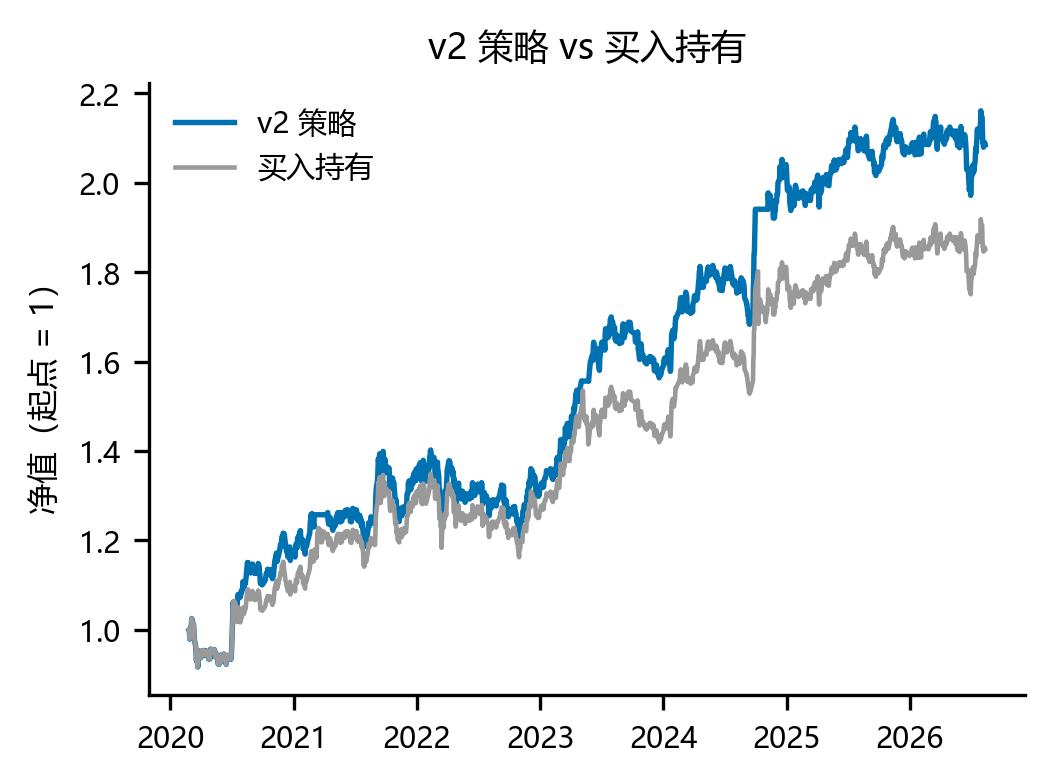
\includegraphics[width=\linewidth]{../figures/fig0_mini_equity.png}

\end{minipage}
\par\vfill

{\color{MemoRule}\hrule height 0.4pt}\medskip
\begin{minipage}[t]{0.36\textwidth}
\vspace{0pt}\small
\setlength{\parskip}{3pt}
\textbf{PREPARED BY}\par\ReportAuthor\par\TeamName\par
\medskip\textbf{COVERAGE}\par\Coverage
\end{minipage}\hfill
\begin{minipage}[t]{0.60\textwidth}
\vspace{0pt}\footnotesize
\setlength{\parskip}{3pt}
\textbf{来源与日期。}数据截至 \DataDate。
信号：data/raw/红利低波50ETF择时信号.xlsx（本人自制，截至 2026-08-12）；
行情：akshare fund\_etf\_hist\_em（东方财富，2026-11-09 抓取，后复权）；
回测输入为 run-002 数据快照（snapshot\_manifest.json 含 SHA-256 与 as\_of）。

\textbf{核验。}33 项单元测试通过；回测前快照哈希复核一致；交易与信号序列对账
一致（抽查 2024-09-27 温度 87.05 \textgreater{} 80，09-30 执行卖出）；报告数值
与 runs/run-002/result/metrics.json 一致。未竟核验：无样本外验证。

\textbf{编制说明。}回测、指标、门禁均为确定性 Python 代码（src/workflow/）；
Kimi Code（LLM 智能体）承担 Generator/Critic 角色、编码与文档整理；规则结构
变更经 H1、终局定稿经 H2 人工裁决；全部数值由代码计算，LLM 无写权限于产物。
\end{minipage}

\clearpage
\normalsize
% 第 2 页正文：策略规则、图表、验收对照、迭代历程、局限与附录
\section*{策略规则（champion v2）与执行细节}
规则类型：单阈值二元择时。每日收盘读取温度计总值：$>$80 目标清仓，
$\leq$80 目标满仓；t 日判定、t+1 收盘执行（收盘价为后复权价）；回测起点
温度 6.82 $\leq$80，立即满仓；仓位二元（100\%/0\%），无现金保留与分档。
成本：佣金单边万 3、双边计提；ETF 无印花税；无滑点（或高估收益，见局限）。

\begin{center}
\captionof{figure}{v2 策略与买入持有净值对比（对数轴；粉色区间为 2022 慢熊，
策略与基线回撤重合）}\label{fig:equity}
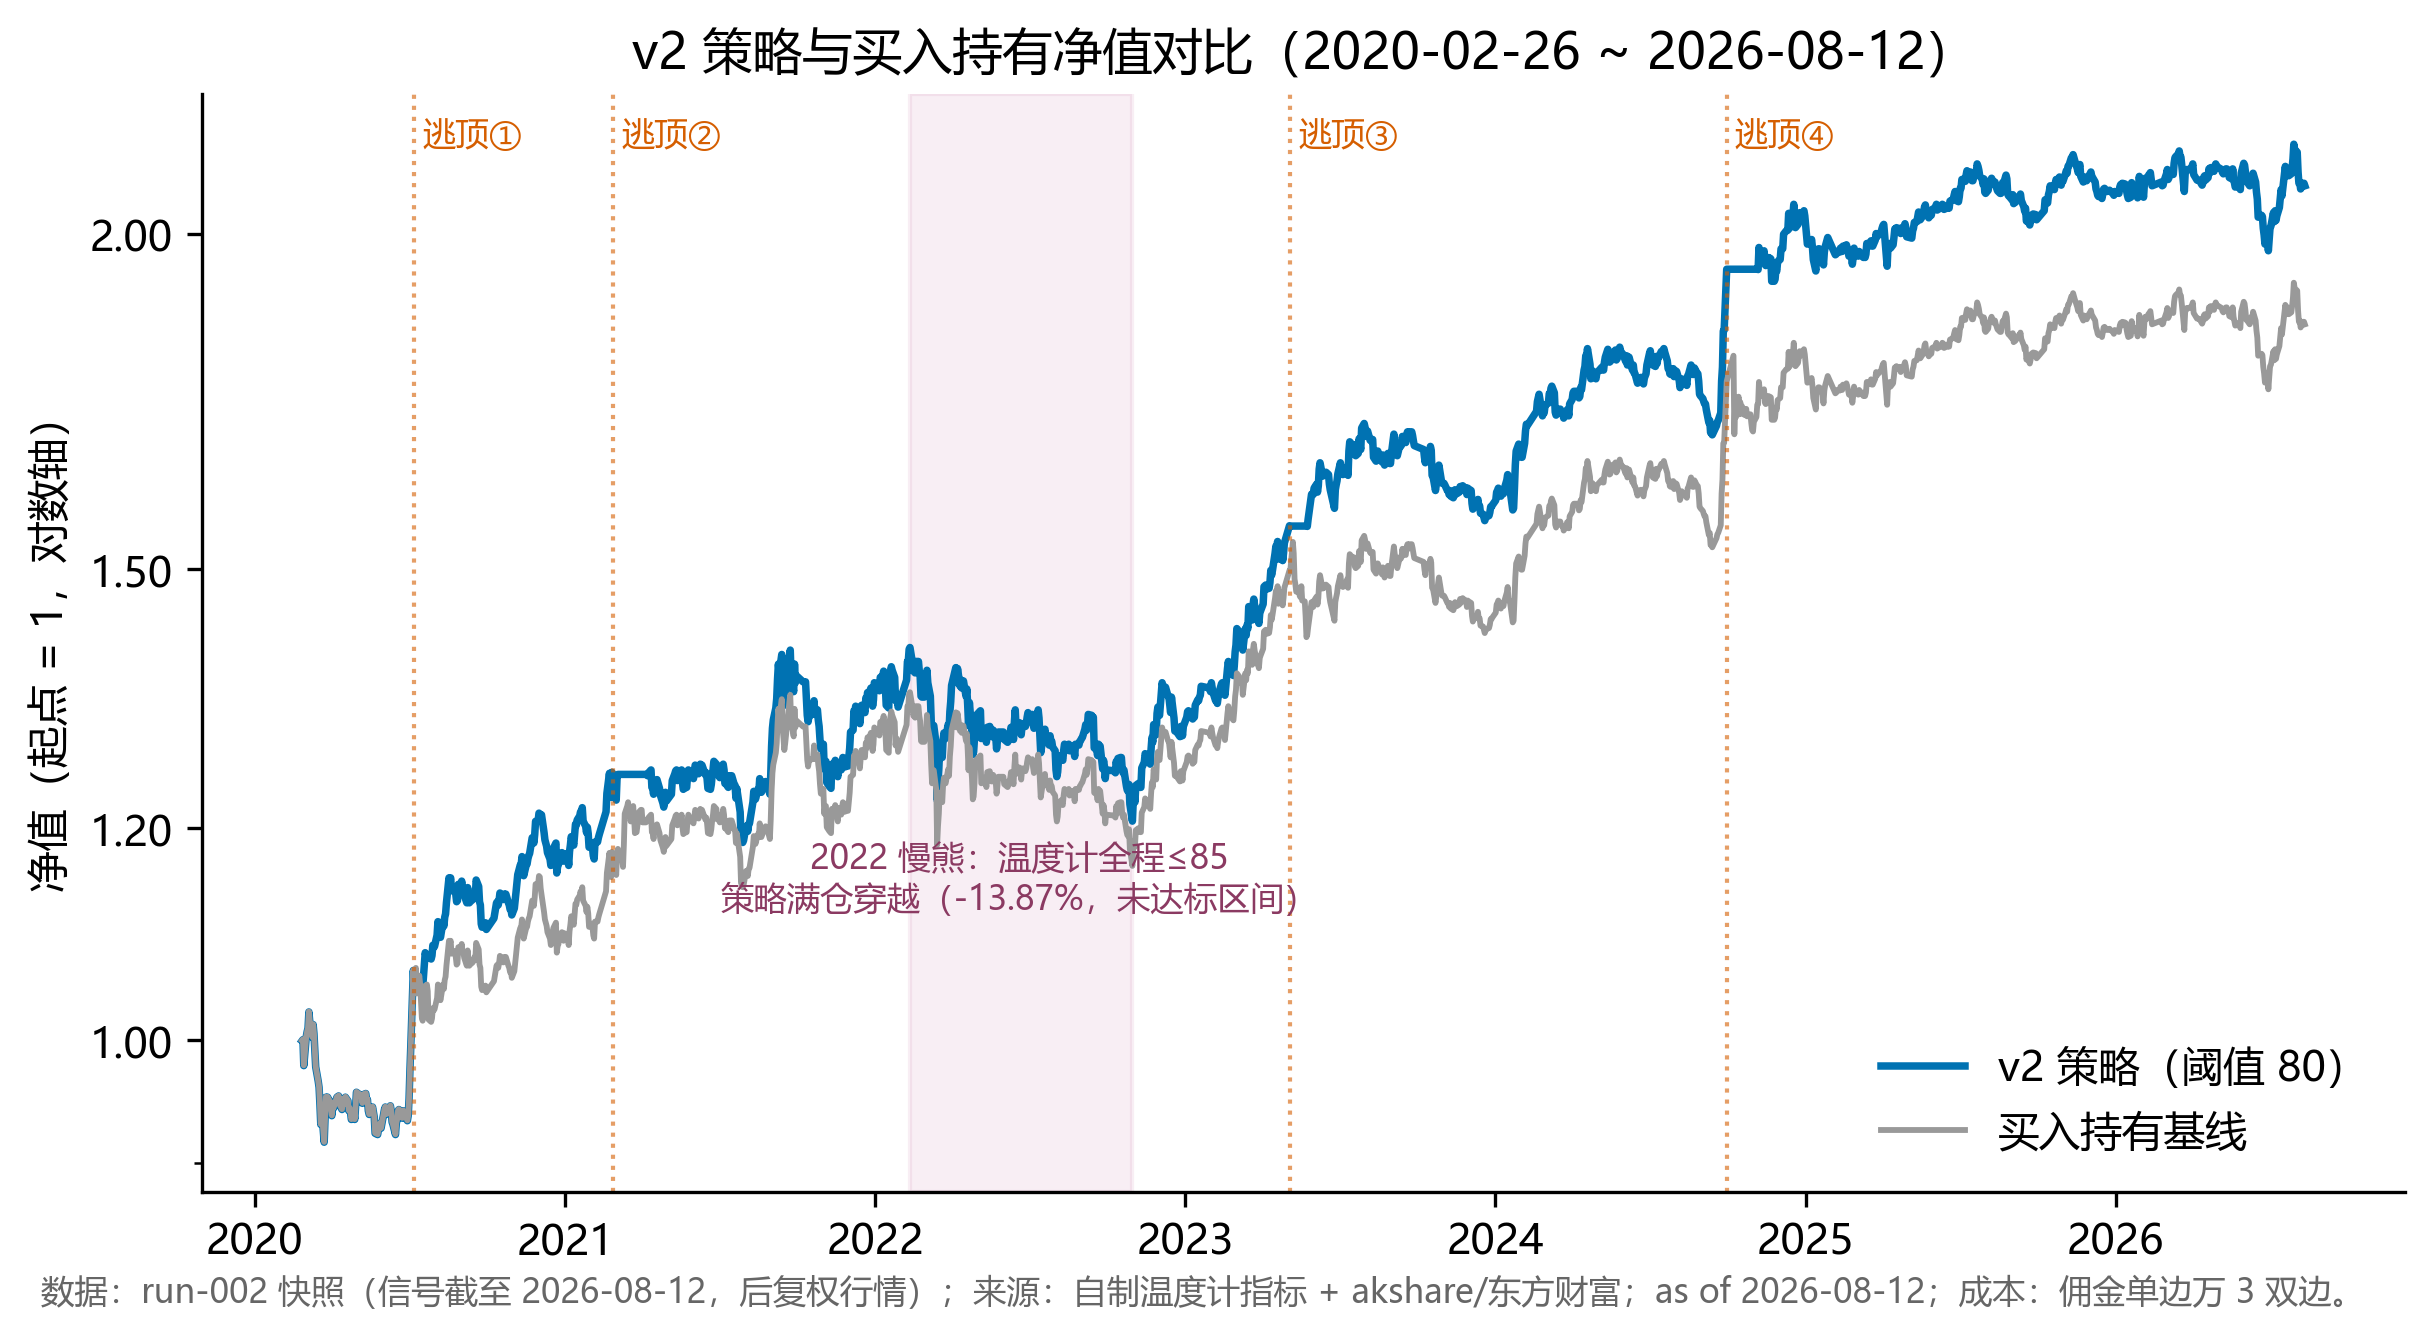
\includegraphics[width=0.86\linewidth]{../figures/fig1_equity.png}
{\footnotesize 来源：run-002 数据快照（信号截至 2026-08-12，后复权行情）；
as of 2026-08-12；成本佣金单边万 3 双边。\par}
\end{center}

\section*{验收对照（task.md 五条标准，对照买入持有基线）}
\begin{center}
\captionof{table}{五条验收标准逐条判定（champion v2，基线同快照重算）}\label{tab:acceptance}
{\footnotesize 判定为确定性代码输出（review/auto\_review.json），LLM 无权更改。\par}
\begin{tabular}{llllc}
\toprule
标准 & 要求 & 基线 & 实际 & 判定 \\
\midrule
1 年化收益 & $\geq$基线$\times$1.05 & 10.42\% & $\geq$10.94\% $\to$ 12.55\% & 达标 \\
2 最大回撤 & $\leq$基线$\times$0.7 & -13.87\% & $\leq$-9.71\% $\to$ -13.87\% & {\color{red}未达标} \\
3 夏普比率 & $\geq$基线$\times$1.2 & 0.8063 & $\geq$0.9676 $\to$ 1.0050 & 达标 \\
4 交易次数 & $\geq$ 10 & --- & 19 & 达标 \\
5 稳健性 & 阈值$\pm$5 结论不反转 & --- & 75--85 五组同判未通过（退化） & 字面达标/实质存疑 \\
\midrule
\multicolumn{5}{l}{综合：五条须全部通过 $\to$ {\color{red}未通过（4/5），如实呈现，不放宽标准}} \\
\bottomrule
\end{tabular}

\end{center}

\section*{三轮迭代历程（假设→证据→裁决）}
\begin{center}
\captionof{table}{run-001/002/003 对照；门禁为确定性数值判定，裁决见各 run critic\_verdict.md}\label{tab:iterations}
{\footnotesize 三 run 共用同一数据快照（SHA-256 一致），"改动净效应"对照成立。\par}
{\small\begin{tabular}{llcccp{3.6cm}}
\toprule
run / 假设 & 规则改动 & 年化/回撤/夏普 & 交易 & 门禁判定 & 被证实/证伪的设计知识 \\
\midrule
run-001 / v1 & 单阈值 85 & 12.21\%/-13.87\%/0.971 & 11 & 未达标（回撤） & 指标只逃顶不防熊 \\
run-002 / v2 & 阈值 85$\to$80 & 12.55\%/-13.87\%/1.005 & 19 & 未达标（回撤） & 调参无解：75--85 回撤全部相同 \\
run-003 / v3 & +MA200 趋势过滤 & 6.53\%/-19.02\%/0.600 & 74 & 未达标（第1/2/3条） & 趋势过滤对低波均值回复品种方向性有害；champion 约束否决 \\
\bottomrule
\end{tabular}
}
\end{center}

过程要点：v1 失败根因（2022 慢熊温度计最高 61.1、全年 0 天 $>$85）在 v2 中得到
"调参无解"的证实（75\textasciitilde{}85 五组回撤清一色 -13.87\%）；v3 结构变更
（H1 批准：叠加 200 日均线趋势过滤）在 2022 年买入每次熊市反弹（全年 -14.6\%
对基线 -3.2\%），回撤反深 5.1 个百分点——同阈值 80 对照 v2 年化 -5.7pp，
champion 单调性约束按设计将其否决。迭代预算 3/5 轮，余 2 轮按"防过拟合单一
样本"主动放弃（H2 裁决）。

\begin{center}
\captionof{figure}{温度计信号与 v2 交易点：卖出全部落在温度尖峰（逃顶有效），
2022 年低位游走无信号（防熊缺位）}\label{fig:temp}
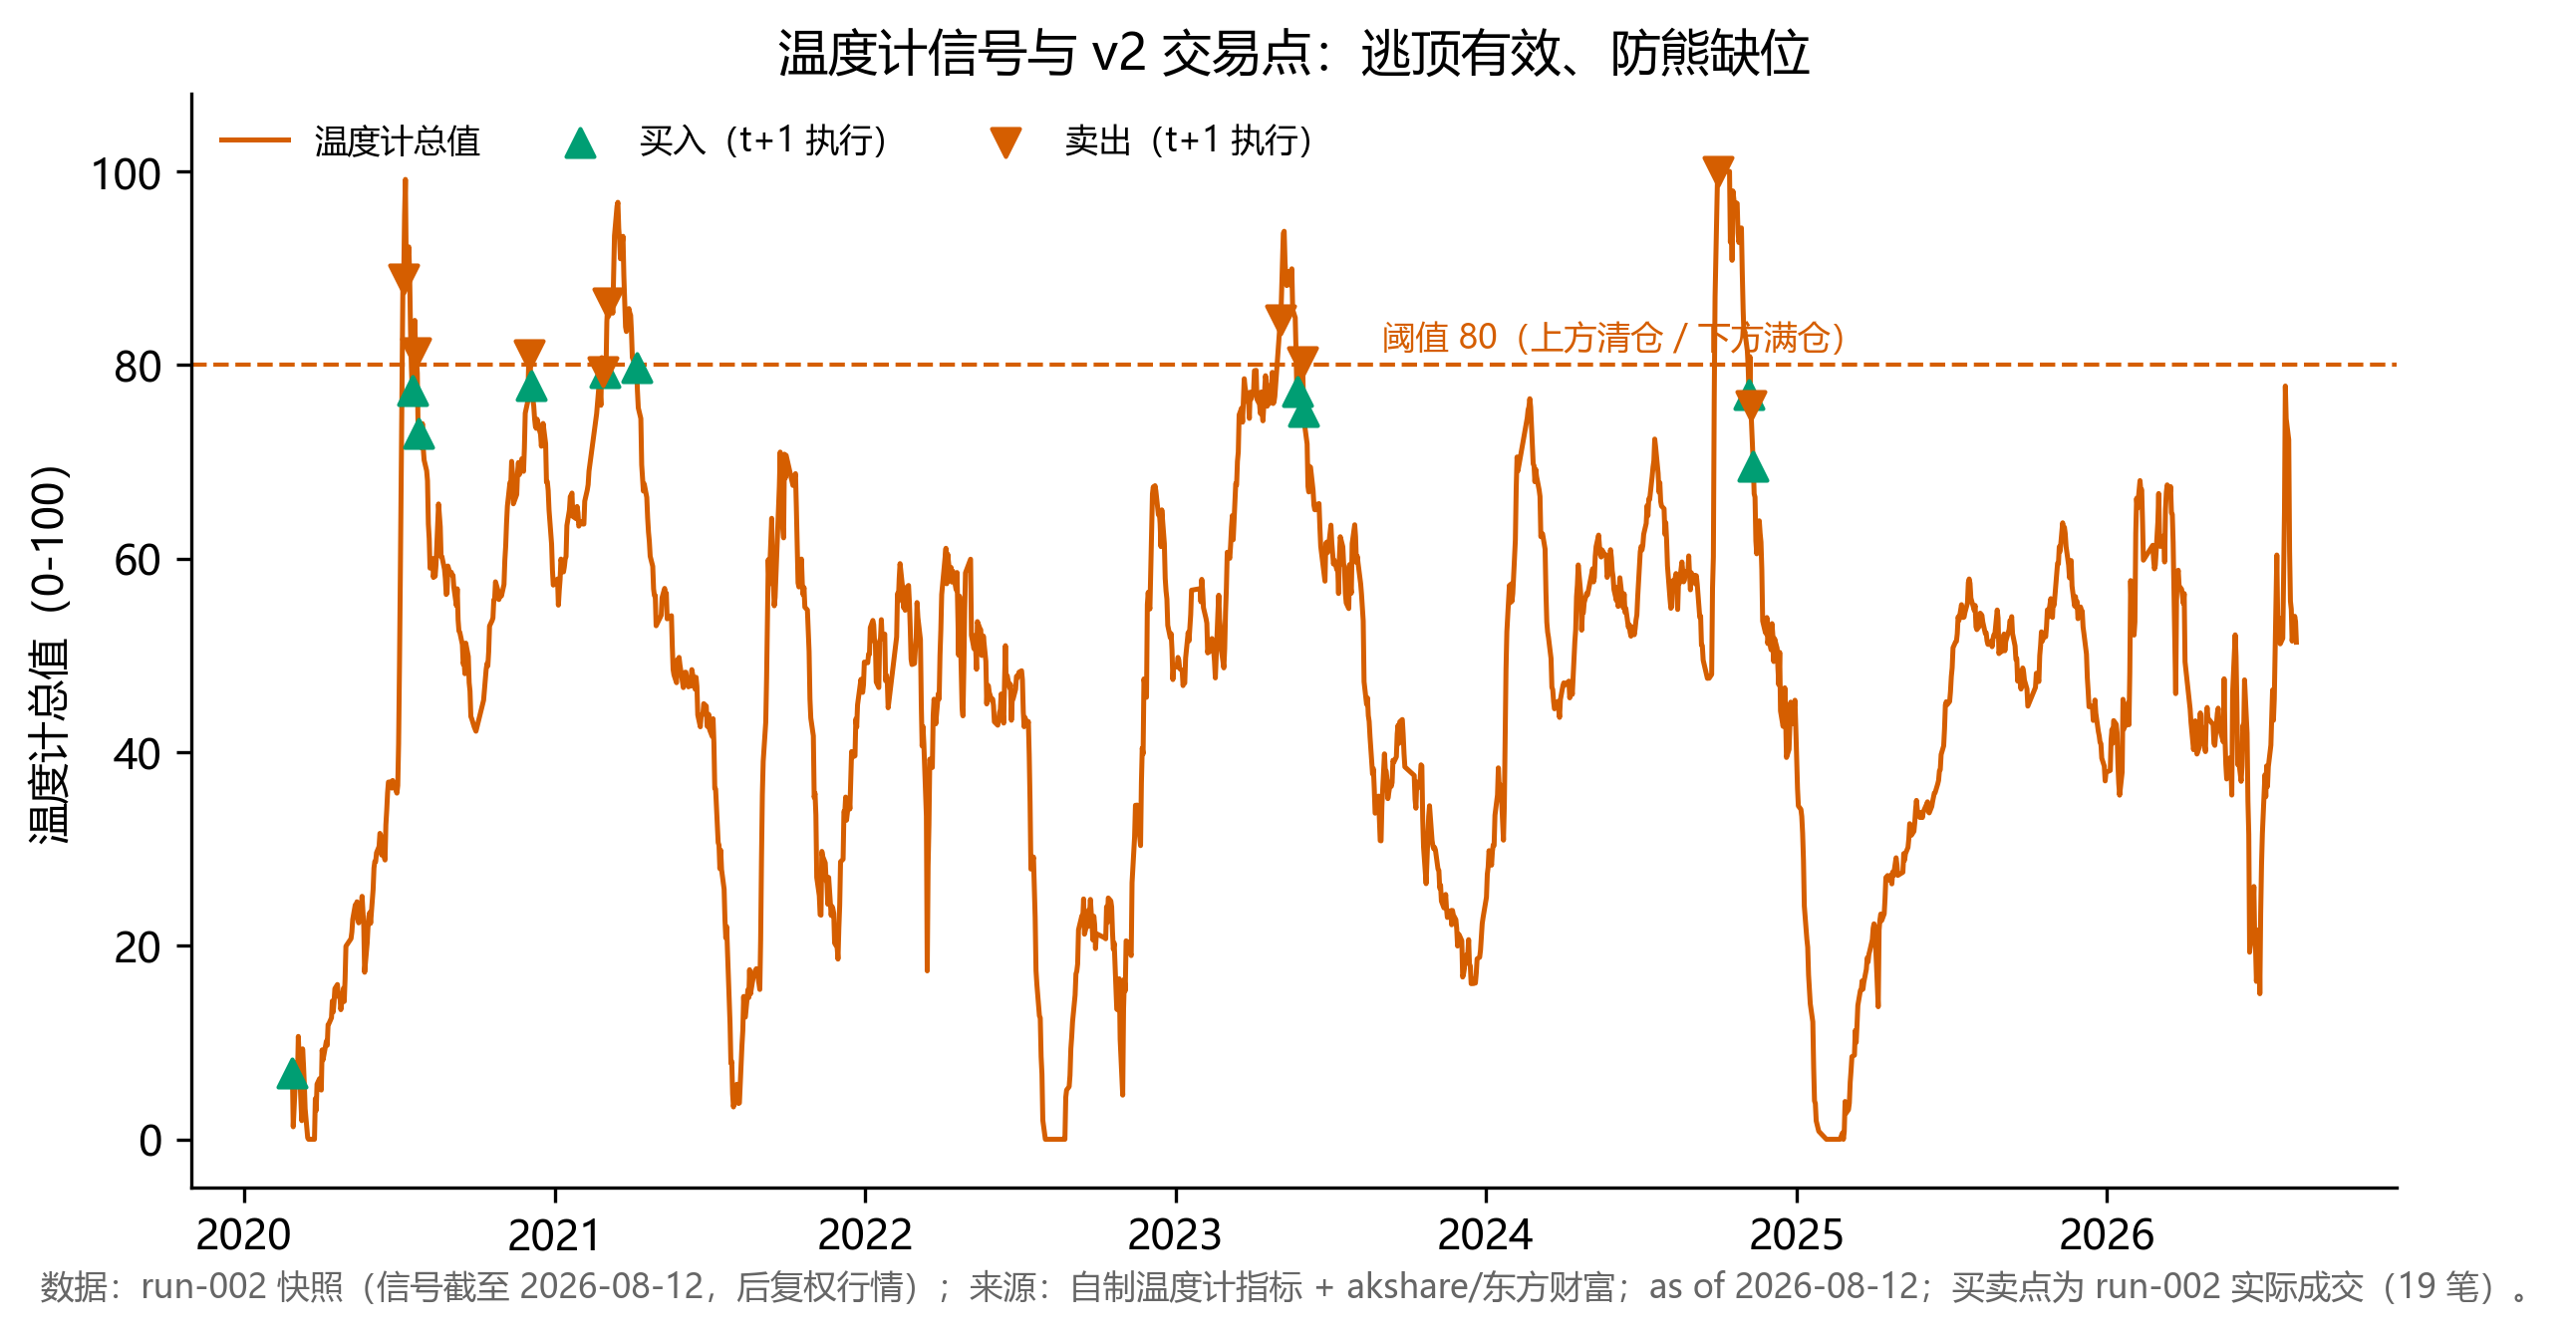
\includegraphics[width=0.86\linewidth]{../figures/fig3_temp_trades.png}
{\footnotesize 来源：run-002 数据快照；买卖点为 19 笔实际成交（t+1 执行）。\par}
\end{center}

\begin{center}
\captionof{figure}{回撤对照：-9.71\% 为验收上限（基线回撤$\times$0.7）；
2022 区间两者回撤曲线重合触底 -13.87\%，第 2 条不达标直证}\label{fig:drawdown}
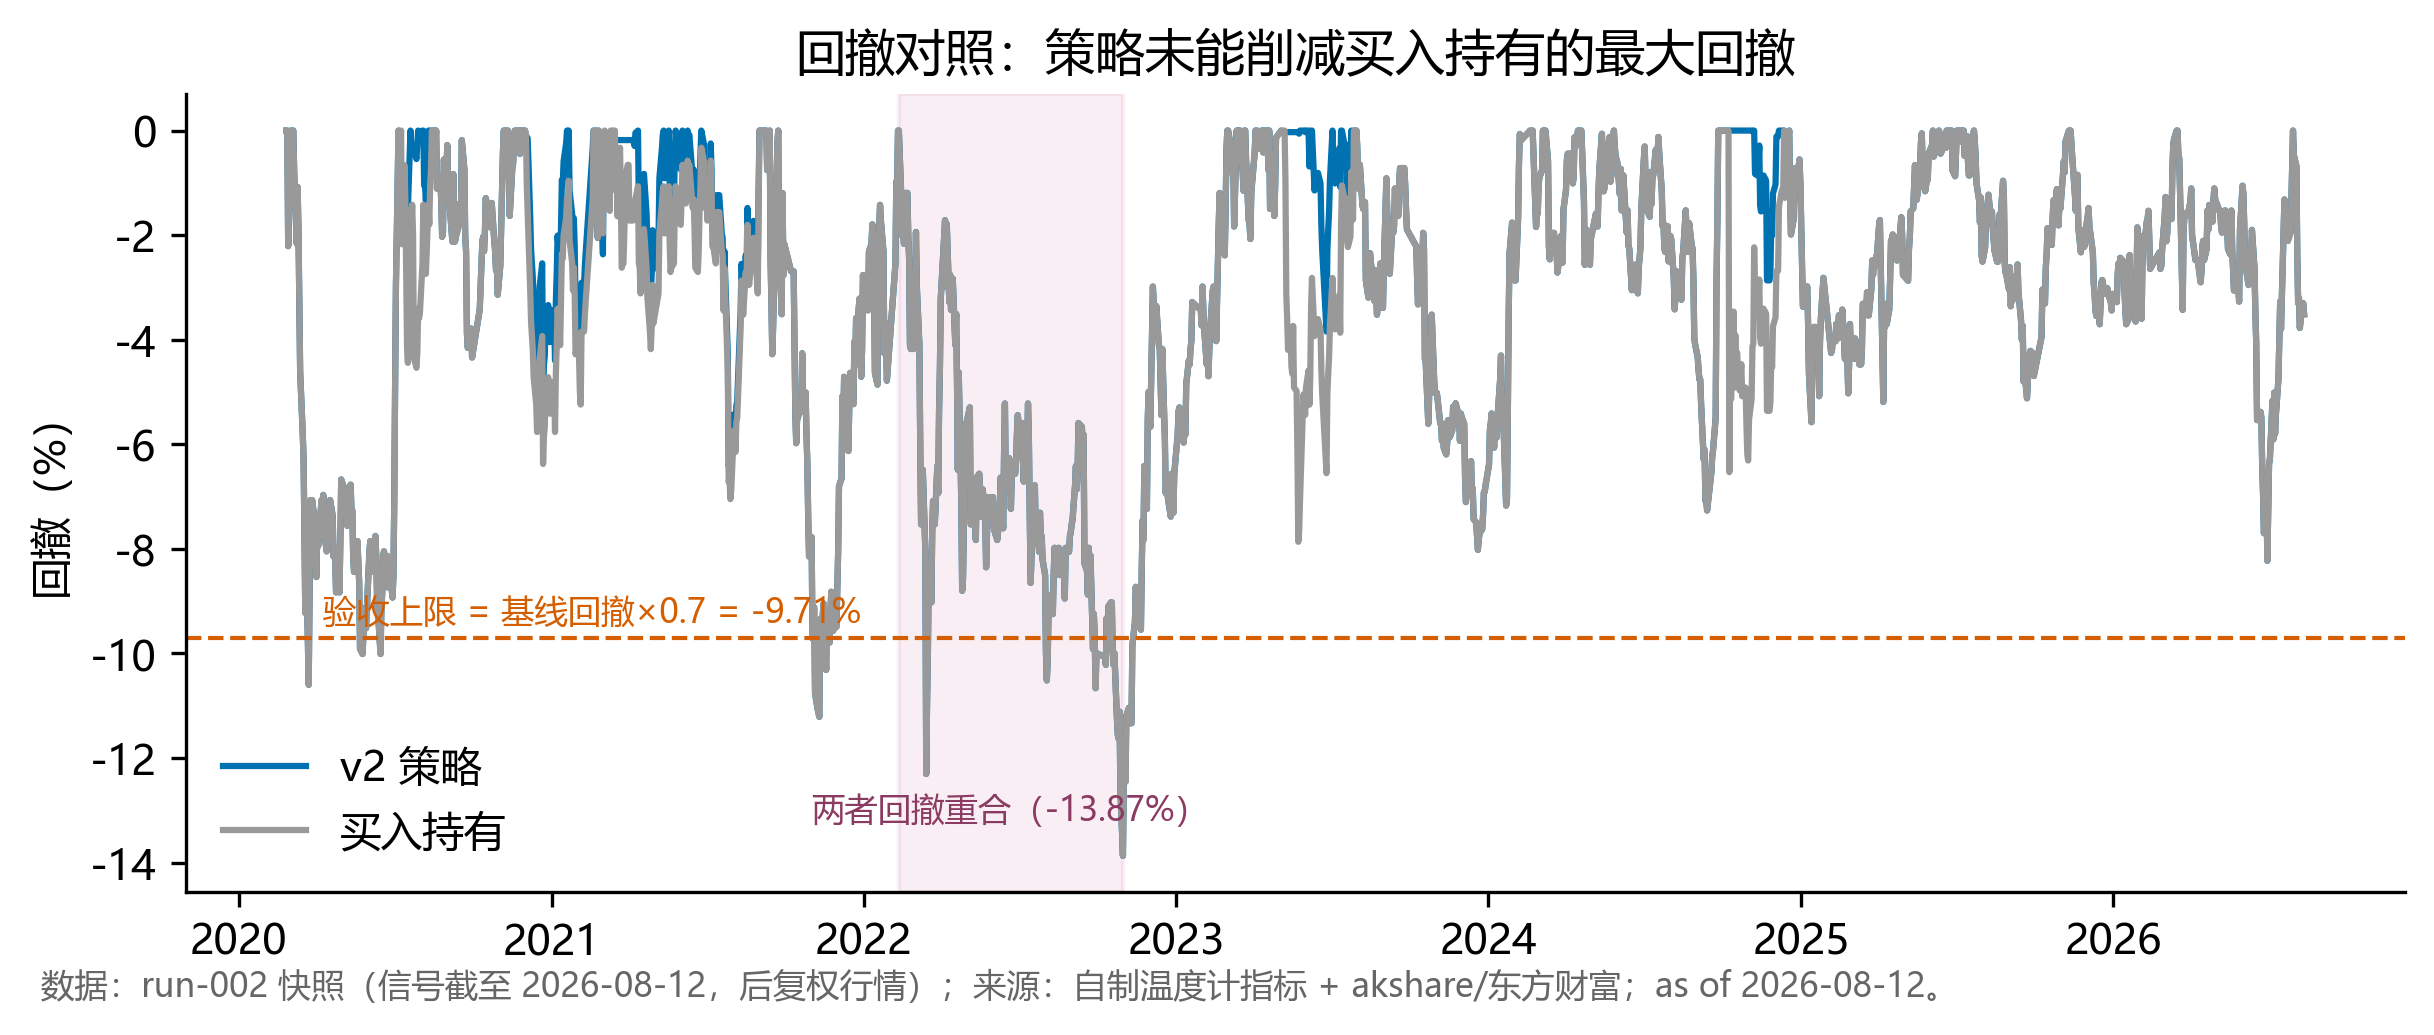
\includegraphics[width=0.8\linewidth]{../figures/fig2_drawdown.png}
{\footnotesize 来源：run-002 数据快照。\par}
\end{center}

\section*{局限与诚实结论}
\begin{itemize}\setlength{\itemsep}{2pt}
  \item \textbf{结论按验收规则为未通过}（4/5）：第 2 条最大回撤 -13.87\%，
        与基线相同，未达 $\leq$ 基线$\times$0.7 的标准；不因其余四条达标而修饰。
  \item 单窗口样本内评估，无样本外验证；窗口仅含一次深熊（2022），
        对该样本继续修规则有过拟合之嫌——这是主动放弃剩余 2 轮预算的理由。
  \item 成本简化为无滑点、免最低佣金，或小幅高估策略收益；权益比例记账
        未按 100 股整手取整。
  \item 稳健性"字面达标"属退化意义（各阈值同判未通过），不构成参数可信度。
  \item 温度计为本人自制指标，结论的外部可复现性受制于指标不可得。
  \item 本报告不构成投资建议；策略为课程作业的研究对象。
\end{itemize}

\section*{附录：文件索引}
任务定义 docs/plans/task.md；架构设计 docs/DESIGN.md 与 docs/workflow.png；
迭代日志 docs/iteration\_log.md；run 状态库 runs/run-001\textasciitilde{}003
（各含 hypothesis.json、data/ 快照与哈希、result/ 指标与敏感性、review/
门禁与裁决）、runs/champion.json；代码 src/workflow/（fetch/backtest/review）、
tests/（33 项单测）；图 docs/figures/、表生成 scripts/make\_report\_tables.py。


\end{document}
